% Editable source for result.pdf, written by make_figures.py from the run's result.json
\documentclass[tikz,border=6pt]{standalone}
\usepackage[T1]{fontenc}
\begin{document}
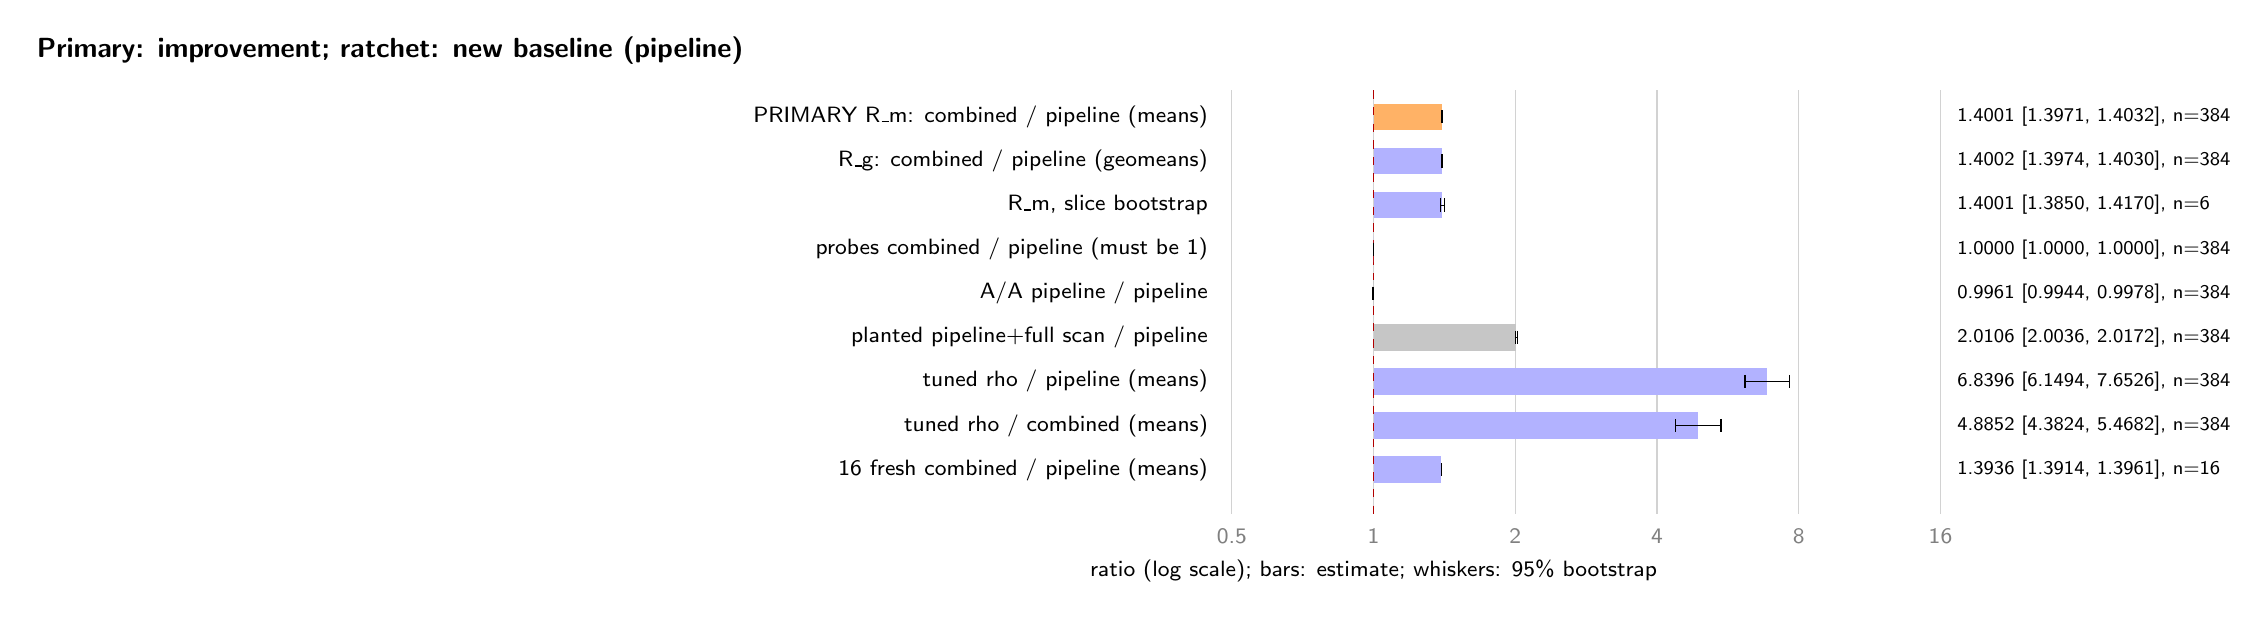
\begin{tikzpicture}[font=\sffamily\footnotesize,x=18mm,y=-5.6mm]
\draw[gray!35] (-1.0000,-0.6) -- (-1.0000,9); \node[gray] at (-1.0000,9.5) {0.5};
\draw[gray!35] (0.0000,-0.6) -- (0.0000,9); \node[gray] at (0.0000,9.5) {1};
\draw[gray!35] (1.0000,-0.6) -- (1.0000,9); \node[gray] at (1.0000,9.5) {2};
\draw[gray!35] (2.0000,-0.6) -- (2.0000,9); \node[gray] at (2.0000,9.5) {4};
\draw[gray!35] (3.0000,-0.6) -- (3.0000,9); \node[gray] at (3.0000,9.5) {8};
\draw[gray!35] (4.0000,-0.6) -- (4.0000,9); \node[gray] at (4.0000,9.5) {16};
\draw[red!70!black,dashed] (0,-0.6) -- (0,9);
\node at (0,10.3) {ratio (log scale); bars: estimate; whiskers: 95\% bootstrap};
\node[anchor=west,font=\sffamily\bfseries] at (-9.5,-1.5) {Primary: improvement; ratchet: new baseline (pipeline)};
\node[anchor=east] at (-1.1000,0) {PRIMARY R\_m: combined / pipeline (means)};
\fill[orange!60] (0,-0.300000) rectangle (0.4855,0.300000);
\draw (0.4825,0) -- (0.4887,0); \draw (0.4825,-0.150000) -- (0.4825,0.150000); \draw (0.4887,-0.150000) -- (0.4887,0.150000);
\node[anchor=west,font=\sffamily\scriptsize] at (4.0500,0) {1.4001 [1.3971, 1.4032], n=384};
\node[anchor=east] at (-1.1000,1) {R\_g: combined / pipeline (geomeans)};
\fill[blue!30] (0,0.700000) rectangle (0.4856,1.300000);
\draw (0.4828,1) -- (0.4885,1); \draw (0.4828,0.850000) -- (0.4828,1.150000); \draw (0.4885,0.850000) -- (0.4885,1.150000);
\node[anchor=west,font=\sffamily\scriptsize] at (4.0500,1) {1.4002 [1.3974, 1.4030], n=384};
\node[anchor=east] at (-1.1000,2) {R\_m, slice bootstrap};
\fill[blue!30] (0,1.700000) rectangle (0.4855,2.300000);
\draw (0.4699,2) -- (0.5029,2); \draw (0.4699,1.850000) -- (0.4699,2.150000); \draw (0.5029,1.850000) -- (0.5029,2.150000);
\node[anchor=west,font=\sffamily\scriptsize] at (4.0500,2) {1.4001 [1.3850, 1.4170], n=6};
\node[anchor=east] at (-1.1000,3) {probes combined / pipeline (must be 1)};
\fill[blue!30] (0,2.700000) rectangle (0.0000,3.300000);
\draw (0.0000,3) -- (0.0000,3); \draw (0.0000,2.850000) -- (0.0000,3.150000); \draw (0.0000,2.850000) -- (0.0000,3.150000);
\node[anchor=west,font=\sffamily\scriptsize] at (4.0500,3) {1.0000 [1.0000, 1.0000], n=384};
\node[anchor=east] at (-1.1000,4) {A/A pipeline / pipeline};
\fill[gray!45] (0,3.700000) rectangle (-0.0056,4.300000);
\draw (-0.0081,4) -- (-0.0031,4); \draw (-0.0081,3.850000) -- (-0.0081,4.150000); \draw (-0.0031,3.850000) -- (-0.0031,4.150000);
\node[anchor=west,font=\sffamily\scriptsize] at (4.0500,4) {0.9961 [0.9944, 0.9978], n=384};
\node[anchor=east] at (-1.1000,5) {planted pipeline+full scan / pipeline};
\fill[gray!45] (0,4.700000) rectangle (1.0076,5.300000);
\draw (1.0026,5) -- (1.0124,5); \draw (1.0026,4.850000) -- (1.0026,5.150000); \draw (1.0124,4.850000) -- (1.0124,5.150000);
\node[anchor=west,font=\sffamily\scriptsize] at (4.0500,5) {2.0106 [2.0036, 2.0172], n=384};
\node[anchor=east] at (-1.1000,6) {tuned rho / pipeline (means)};
\fill[blue!30] (0,5.700000) rectangle (2.7739,6.300000);
\draw (2.6204,6) -- (2.9360,6); \draw (2.6204,5.850000) -- (2.6204,6.150000); \draw (2.9360,5.850000) -- (2.9360,6.150000);
\node[anchor=west,font=\sffamily\scriptsize] at (4.0500,6) {6.8396 [6.1494, 7.6526], n=384};
\node[anchor=east] at (-1.1000,7) {tuned rho / combined (means)};
\fill[blue!30] (0,6.700000) rectangle (2.2884,7.300000);
\draw (2.1317,7) -- (2.4511,7); \draw (2.1317,6.850000) -- (2.1317,7.150000); \draw (2.4511,6.850000) -- (2.4511,7.150000);
\node[anchor=west,font=\sffamily\scriptsize] at (4.0500,7) {4.8852 [4.3824, 5.4682], n=384};
\node[anchor=east] at (-1.1000,8) {16 fresh combined / pipeline (means)};
\fill[blue!30] (0,7.700000) rectangle (0.4788,8.300000);
\draw (0.4765,8) -- (0.4814,8); \draw (0.4765,7.850000) -- (0.4765,8.150000); \draw (0.4814,7.850000) -- (0.4814,8.150000);
\node[anchor=west,font=\sffamily\scriptsize] at (4.0500,8) {1.3936 [1.3914, 1.3961], n=16};
\end{tikzpicture}
\end{document}
